\documentclass[a4paper,11pt]{article}

\usepackage[utf8]{inputenc}
\usepackage{times}           
\usepackage[french]{babel}

\usepackage{graphicx}
\usepackage{amsmath, amsthm, amssymb}  
\usepackage{url}

\sloppy

\title{DM d'algo parallèle}
\author{Baptiste Rozière et Alice Pellet-Mary}
\date{\today} 

\begin{document}

\maketitle

\section*{Question 3}


\section*{Question 5}
L'automate est bien définit si on n'a pas dans DEP à la fois nord et sud, ou bien à la fois ouest et est. Si on a nord et sud ou est et ouest, on aura une boucle, chaque case devra se mettre à jour après ses voisins qui devront eux même se mettre à jour après elle.
En revanche, si on n'a pas à la fois nord et sud ou à la fois est et ouest, l'automate sera bien défini car les lignes et colonnes des bords n'ont pas de voisins, donc elles pourront se mettre à jour sans attendre que d'autres cases se mettent à jour.\\
Si la première et dernière ligne sont voisines, on ne peut plus faire de dépendances nord ou sud. Les seuls cas où DEP sera bien défini seront $DEP = \{E\}$, $DEP = \{W\}$ ou $DEP = \emptyset$. Si on a $N$ ou $S$ dans $DEP$, par exemple $N$, la première ligne aura besoin de la dernière pour se mettre à jour, qui aura besoin de l'avant dernière, ..., qui aura besoin de la première. Donc l'automate n'est plus bien défini.\\
Dans le cas où la première et la dernière colonne sont voisines aussi, il n'y a plus aucune dépendance possible. Le seul cas où l'automate sera bien défini est le cas $DEP = \emptyset$.


\section*{Question 6}
On peut trouver un algorithme efficace équivalent à l'algorithme séquentiel si les dépendances sont $DEP = \{N\}$, $DEP = \{W\}$ ou $DEP = \{N, W\}$. Dans les cas où on a $S$ ou $E$ dans les dépendances, on ne peut pas appliquer l'algorithme séquentiel, car comme on va de haut en bas et de gauche à droite, lorsqu'on veut mettre à jour une case, il n'y a que les cases au nord et à l'est qui ont été modifiées. On ne peut donc pas prendre en compte les modifications des cases à l'est et au sud.\\
Dans le cas où $DEP = \{N\}$, on a un algorithme parallèle efficace en pipelinant les calculs. On distribue la matrice entre les processeurs comme sur le dessin (un bloc de matrice par processeur).
\begin{figure}[!h]
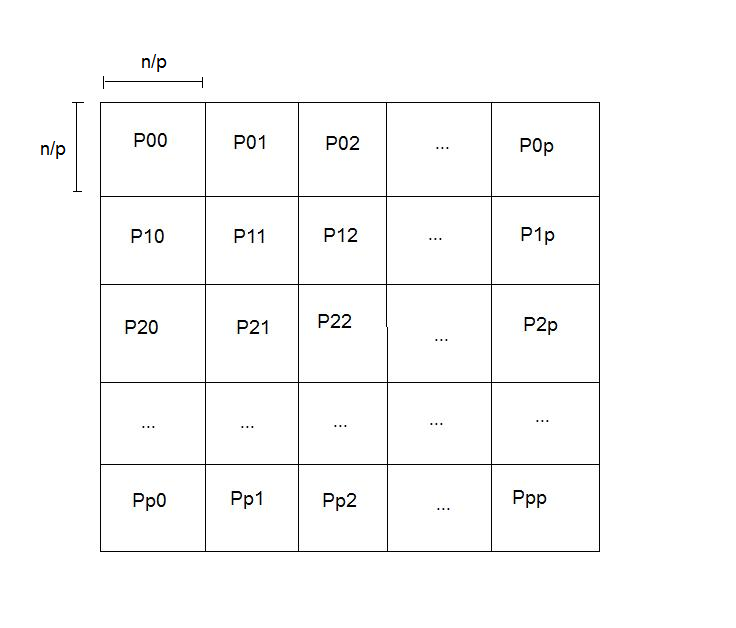
\includegraphics[scale=0.4]{repartition.png}
\caption{répartition de la matrice sur les processeurs}
\label{repartition}
\end{figure}
\\Les blocs du haut mettent à jour la première ligne de leur bloc, et envoient le résultat de la dernière case de leur première ligne au bloc en dessous, qui peuvent alors commencer à calculer les valeurs de leur première ligne pendant que le bloc du dessus calcule les valeurs de sa deuxième ligne et ainsi de suite (cf figure~\ref{etapes}).
\begin{figure}[!h]
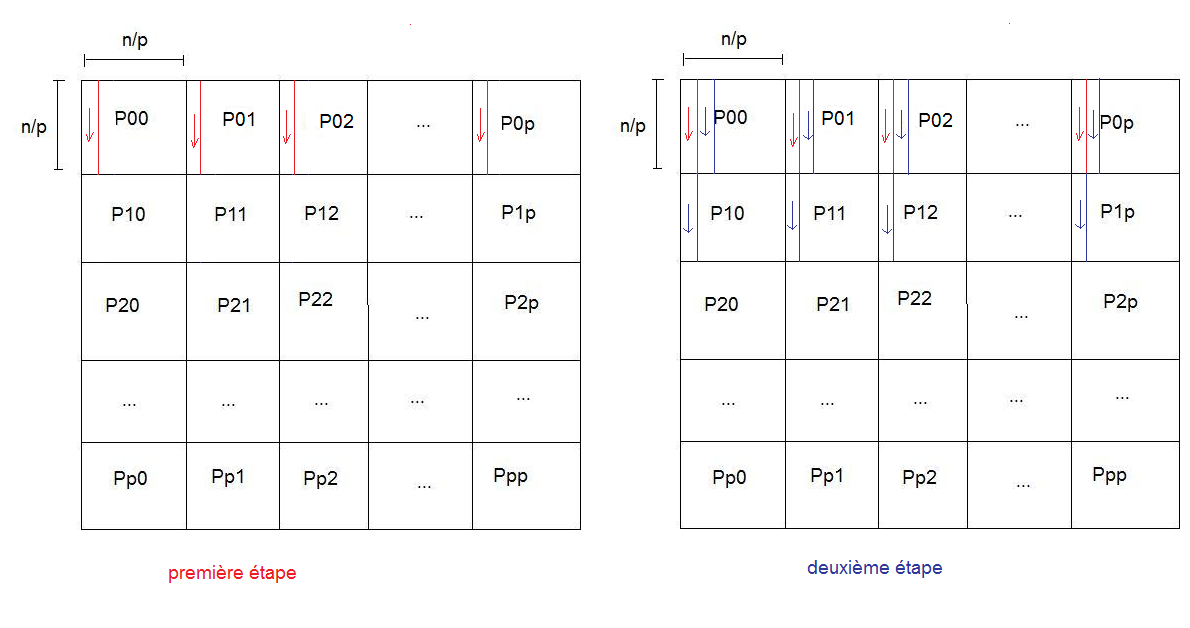
\includegraphics[scale=0.4]{etapes.png}
\caption{mise à jour des éléments}
\label{etapes}
\end{figure}
\\
Si on veut faire plusieurs mises à jours, les blocs du haut peuvent commencer la deuxième mise à jour une fois qu'ils ont fini de mettre à jour toutes leurs cellules. Comme ça les processeurs n'ont pas de moments oisifs à part au début lorsqu'ils attendent leurs premières données.\\
Si $DEP = \{E\}$, l'idée est la même.\\
Si $DEP = \{N,W\}$, on fait les calculs diagonales par diagonales (cf figure~\ref{diagonales}).
On peut optimiser le temps de calcul en modifiant l'ordre de calcul dans les blocs, pour que les blocs voisins puissent commencer à travailler le plus tôt possible.
\begin{figure}[!h]
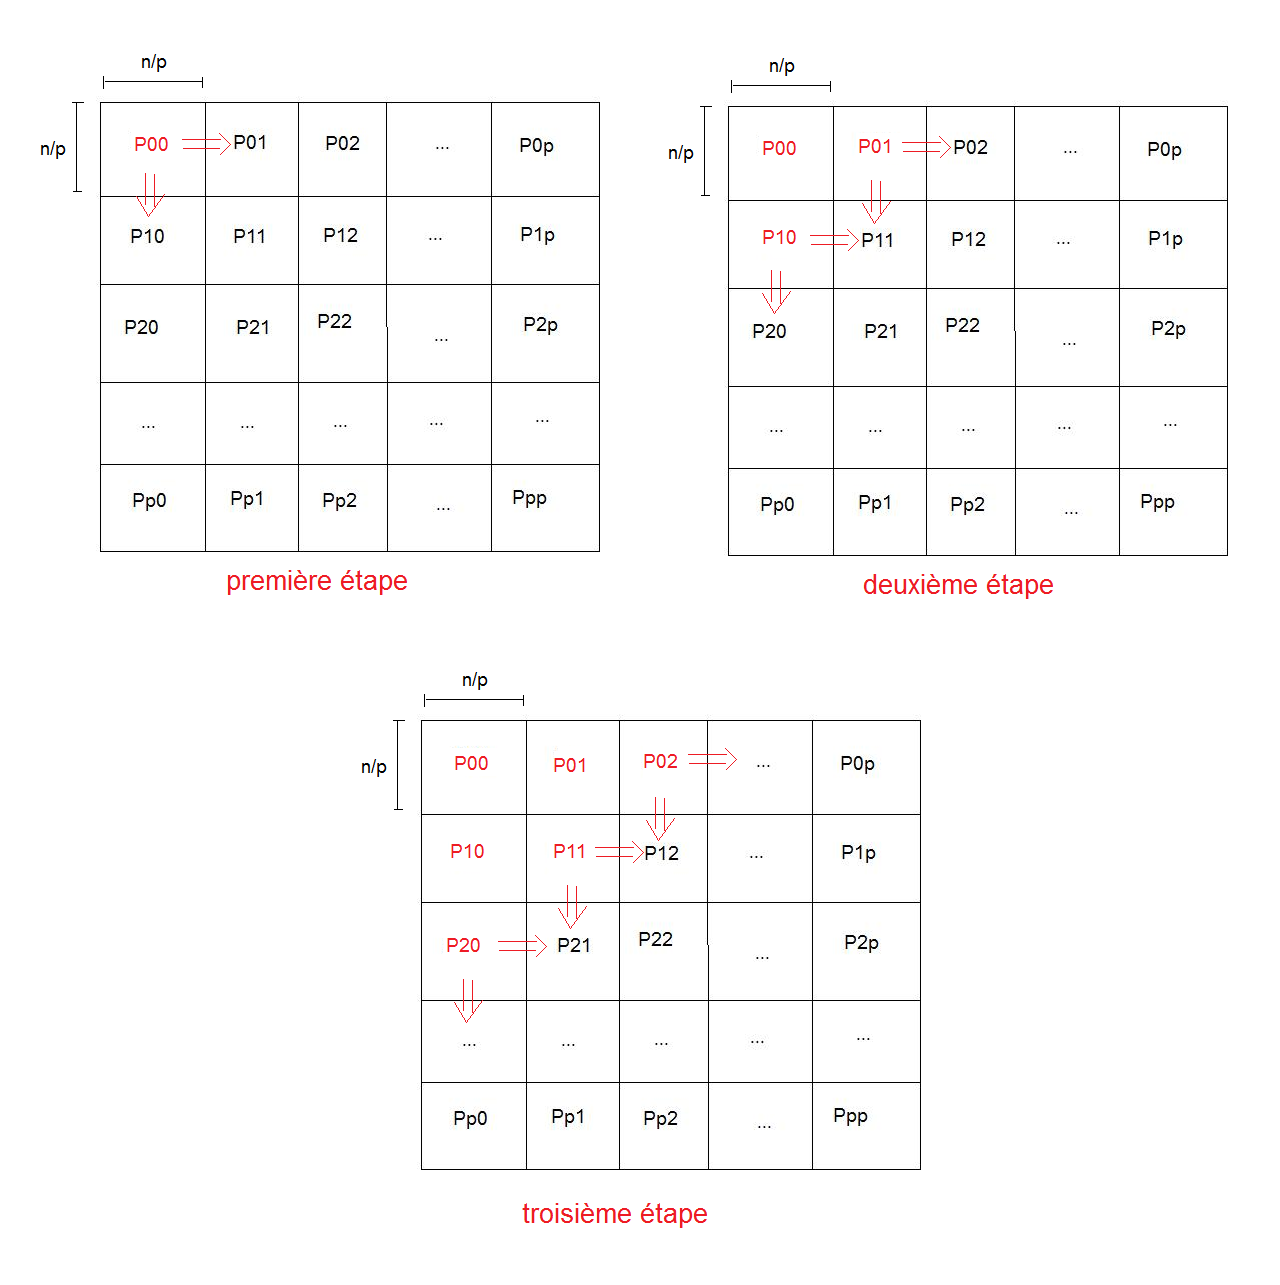
\includegraphics[scale=0.4]{diagonales.png}
\caption{$DEP = \{N,W\}$}
\label{diagonales}
\end{figure}
\\
\\
Si maintenant on a une topologie d'anneau, on peut toujours trouver des algorithmes efficaces. Par exemple si $DEP = \{N\}$, on attribue à chaque processeur un bloc de colonne, et ils font tous leurs calculs en parallèle sans avoir besoin de communiques (cf figure \ref{anneau1}).
\begin{figure}[!h]
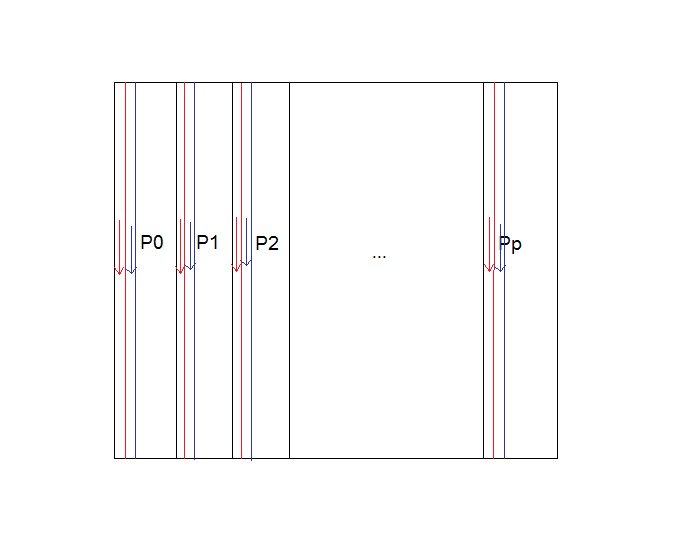
\includegraphics[scale=0.5]{anneau1.png}
\caption{topologie d'anneau et $DEP = \{N\}$}
\label{anneau1}
\end{figure}
De même si $DEP = \{W\}$ on attribue des blocs de lignes à chaque processeur.\\
Si $DEP = \{N,W\}$, on attribue des blocs de colonnes à chaque processeur, le premier calcule la première ligne puis envoie son dernier élément au deuxième, qui peut alors calculer sa première ligne, pendant que le première processeur calcule sa deuxième ligne et ainsi de suite (cd figure \ref{anneau2}).
\begin{figure}[!h]
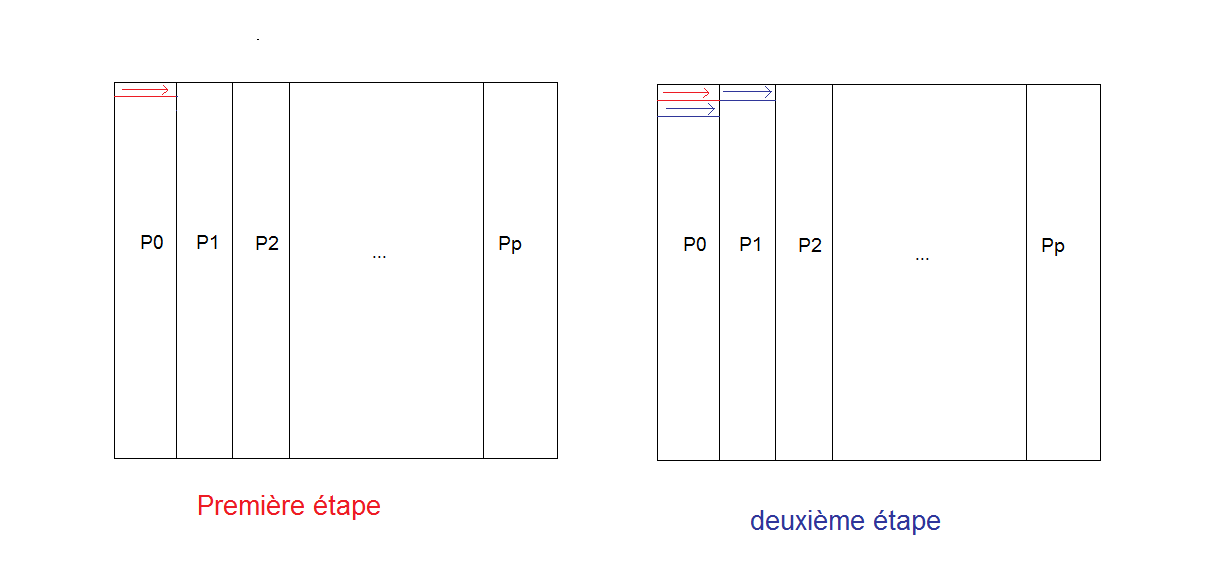
\includegraphics[scale=0.5]{anneau2.png}
\caption{topologie d'anneau et $DEP = \{N,W\}$}
\label{anneau2}
\end{figure}

\section*{Question 8}



\end{document}